%!TEX root = ../luanvan.tex
\chapter{Cơ sở lý thuyết}
\section{Quản lý văn bằng chứng chỉ}
\subsection{Giới thiệu}

Xã hội ngày càng phát triển nên nhu cầu học tập nâng cao trình độ đáp ứng cho các lĩnh vực lao động xã hội ngày càng tăng.
Hàng năm có hàng nghìn các loại văn bằng, chứng chỉ được cấp phát để công nhận trình độ, năng lực của các học viên đã qua một quá trình học tập và thi đạt.
Ngoài ra, văn bằng được dùng trong tuyển dụng lao động và làm thủ tục hồ sơ liên quan khác, ảnh hưởng nhiều đến người sở hữu trong tương lai.
Trong nhiều ngành nghề, chứng chỉ là điều kiện để thực hiện công việc, có tính quyết định và ảnh hưởng tới nhiều lĩnh vực khác.
Do đó, quản lý văn bằng chứng chỉ đòi hỏi quy trình thực hiện nghiêm ngặt, tránh những trường hợp lợi dụng kẽ hở để thực hiện hành vi trái pháp luật.

Một số văn bản pháp luật được ban hành nhằm quy định việc quản lý văn bằng chứng chỉ, đảm bảo quyền lợi, trách nhiệm của các tổ chức và cá nhân như sau:

\begin{itemize}
\item Điều 12 Luật giáo dục 2019 quy định “Văn bằng của hệ thống giáo dục quốc dân được cấp cho người học sau khi tốt nghiệp cấp học hoặc sau khi hoàn thành chương trình giáo dục, đạt chuẩn đầu ra của trình độ tương ứng theo quy định của Luật giáo dục. Văn bằng của hệ thống giáo dục quốc dân gồm bằng tốt nghiệp trung học cơ sở, bằng tốt nghiệp trung học phổ thông, bằng tốt nghiệp trung cấp, bằng tốt nghiệp cao đẳng, bằng cử nhân, bằng thạc sĩ, bằng tiến sĩ và văn bằng trình độ tương đương. Chứng chỉ của hệ thống giáo dục quốc dân được cấp cho người học để xác nhận kết quả học tập sau khi được đào tạo, bồi dưỡng nâng cao trình độ học vấn, nghề nghiệp hoặc cấp cho người học dự thi lấy chứng chỉ theo quy định.”

\item Điều 3 Thông tư 21/2019/TT-BGDĐT quy định về việc ban hành Quy chế quản lý văn bằng, chứng chỉ của hệ thống giáo dục quốc dân, quy định việc phân cấp và giao quyền tự chủ, tự chịu trách nhiệm trong quản lý văn bằng, chứng chỉ. Cơ sở giáo dục đại học, cơ sở đào tạo giáo viên tự chủ và tự chịu trách nhiệm trong việc quản lý, cấp phát văn bằng, chứng chỉ theo quy định của pháp luật và quy định của Bộ trưởng Bộ Giáo dục và Đào tạo.

\item Điều 5 Nghị định số 30/2020/NĐ-CP quy định về hoạt động văn thư lưu trữ, giá trị pháp lý về hồ sơ điện tử, văn bản điện tử được ký số bởi người có thẩm quyền và ký số của cơ quan, tổ chức theo quy định của pháp luật có giá trị pháp lý như bản gốc văn bản giấy.

\item Nghị định Số 45/2020/NĐ-CP quy định thủ tục hành chính trên môi trường điện tử. Thủ tục hồ sơ điện tử rất tiết kiệm thời gian và thuận tiện hơn hình thức còn lại nên các giao dịch điện tử tăng nhanh trong những năm gần đây: thanh toán trực tuyến, nộp thuế qua mạng, hóa đơn điện tử, dịch vụ công trực tuyến.
\end{itemize}

Từ năm học 2020-2021, Bộ Giáo dục và Đào tạo đã triển khai ứng dụng công nghệ để lưu trữ văn bằng quốc gia. Hệ thống ứng dụng công nghệ blockchain được triển khai bởi nhà phát triển công nghệ TomoChain. Hiệu quả của hệ thống được khẳng định là đảm bảo tính minh bạch, an toàn và tiết kiệm xã hội. Các đơn vị đào tạo thuộc Bộ Giáo dục và Đào tạo sẽ đưa dữ liệu văn bằng được cấp bởi các đơn vị vào hệ thống lưu trữ văn bằng quốc gia. Bên cạnh đó hệ thống còn đáp ứng những yêu cầu truy xuất cho các bên có nhu cầu và được xã hội hoá.

Học viện Công nghệ Bưu chính Viễn thông đang triển khai thí điểm Cổng thông tin xác thực văn bằng chứng chỉ trên môi trường số với nền tảng ứng dụng công nghệ Blockchain và chữ ký số. Hệ thống phần mềm đảm bảo tính công khai, minh bạch, tin cậy trong công tác tra cứu và xác thực văn bằng, chứng chỉ; hướng tới việc cấp văn bằng, chứng chỉ số trong tương lai đáp ứng theo Nghị định số 30/2020/NĐ-CP. Giải pháp có thể chống lại những hành vi làm giả chứng chỉ, hoặc cấp chứng chỉ không đúng quy định. Hệ thống giúp cho các cơ quan, tổ chức, cá nhân trong quá trình kiểm tra xác minh văn bằng chứng chỉ khi tuyển dụng giảm nhiều thời gian, sức lực so với cách truyền thống.

Trung tâm Tin học Trường Đại học An Giang (gọi tắt là Trung tâm) là đơn vị trực thuộc Trường Đại học An Giang. Từ năm 2017, Trung tâm thực hiện tổ chức thi và cấp chứng chỉ theo Quy chế tổ chức thi và cấp chứng chỉ ứng dụng công nghệ thông tin ban hành theo Quyết định 04/QĐ-TTTH ngày 27/2/2017 của Giám đốc Trung tâm Tin học (gọi tắt là Quy chế). Việc quản lý các dữ liệu chứng chỉ do đơn vị cấp cần phải đảm bảo tính chính xác. Hai hình thức giao dịch giữa các đơn vị trong và ngoài tổ chức; và giữa đơn vị với cá nhân bằng hồ sơ điện tử và hồ sơ sơ giấy. Tuy nhiên, phạm vi nghiên cứu của đề tài chỉ tập trung vào hình thức hồ sơ giấy trong công tác tổ chức thi và cấp chứng chỉ như công văn, quyết định, phôi chứng chỉ và sổ gốc cấp chứng chỉ.

Theo đó, quản lý văn bằng chứng chỉ tại Trung tâm là triển khai các ban hành, phổ biến thông tin, tiếp nhận yêu cầu, thực hiện và lưu giữ hồ sơ được quy định tại Quy chế tổ chức thi và cấp chứng chỉ ứng dụng công nghệ thông tin ban hành theo Quyết định 04/QĐ-TTTH ngày 27/2/2017, bao gồm các nội dung như sau:

\begin{enumerate}
\item Kiểm tra thông tin học viên được cấp chứng chỉ
\item Gửi công văn đề nghị cấp phôi chứng chỉ
\item Tiếp nhận và quản lý phôi chứng chỉ
\item Lập sổ gốc
\item In chứng chỉ
\item Cấp phát chứng chỉ
\item Bảo quản chứng chỉ
\item Xác minh chứng chỉ
\item Cấp giấy xác nhận kết quả thi đạt
\item Thu hồi, hủy bỏ chứng chỉ
\end{enumerate}

Trong phạm vi khả năng giới hạn, đề tài tập trung nghiên cứu vào việc lưu trữ thông tin văn bằng chứng chỉ dùng công nghệ blockchain để tăng tính bảo mật và chắc chắn cho việc cấp phát các văn bằng, chứng chỉ cho học viên sử dụng. Dữ liệu đầu vào của hệ thống được nhập vào từ chương trình quản lý học, quản lý thi. Những chương trình này được đã triển khai và đang đáp ứng tốt một số nghiệp vụ quản lý hiện nay. Đề tài nghiên cứu những nghiệp vụ như sau:

\begin{itemize}
\item Cấp phát chứng chỉ
\item Xác minh chứng chỉ
\end{itemize}

\subsection{Cấp phát chứng chỉ}

Việc cấp phát chứng chỉ được quy định tại Điều 17 của Quy chế và Điều 19 Thông tư 21/2019/TT-BGDĐT. Sổ gốc cấp văn bằng, chứng chỉ phải được ghi chính xác, đánh số trang, đóng dấu giáp lai, không được tẩy xóa, đảm bảo quản lý chặt chẽ và lưu trữ vĩnh viễn.

\begin{enumerate}
\item Thí sinh thi đạt sẽ được cấp chứng chỉ. Sinh viên trực tiếp nhận và đem theo thẻ sinh viên hoặc chứng minh nhân dân, căn cước công dân hoặc giấy tờ có ảnh. Hoặc người được ủy quyền đến trực tiếp nhận và có đem theo giấy tờ tương tự.
\item Nhân viên dựa vào hệ thống quản lý và sổ gốc cấp chứng chỉ để kiểm tra thông tin chứng chỉ.
\item Nếu thông tin sinh viên trùng khớp trong sổ gốc cấp chứng chỉ thì nhân viên sẽ ghi lại thông tin người nhận vào sổ gốc cấp chứng chỉ.
\item Nhân viên phát chứng chỉ cho người nhận.
\item Sinh viên ký tên xác nhận thông tin đó.
\end{enumerate}

\subsection{Xác minh chứng chỉ}

Việc xác minh văn bằng, chứng chỉ là một trong những giai đoạn cần thực hiện để phát hành văn bản có hiệu lực. Quy trình xác minh văn bằng, chứng chỉ là một dạng thủ tục hành chính, cơ sở đào tạo xác minh thông tin chứng chỉ với sổ gốc, kết quả thủ tục là đơn vị yêu cầu xác minh sẽ nhận được công văn trả lời kết quả xác minh (không phải là khẳng định chứng chỉ có giá trị hay không). Quy trình này trải qua 5 bước thực hiện chính như sau:

\begin{enumerate}
\item Đơn vị có nhu cầu xác minh các văn bằng, chứng chỉ cần gửi công văn đến cơ sở đào tạo. Đơn vị có thể cử người có giấy giới thiệu đến trực tiếp phòng ban để bắt đầu làm thủ tục xác minh. Trong quá trình gửi công văn, đơn vị phải chịu trách nhiệm với hồ sơ được bàn giao.
\item Người phụ trách xác minh tại cơ sở tổ chức thi khi tiếp nhận hồ sơ gửi đến sẽ tiến hành kiểm tra lại hồ sơ, và thông tin trong sổ gốc được lập từ trước. Xác nhận người nhận chứng chỉ có trong danh sách thi, đã đạt kết quả và có thông tin chứng chỉ trong sổ gốc.
\item Người phụ trách kiểm tra xác nhận trong sổ gốc xong cần phải soạn công văn, và đề nghị lãnh đạo cơ quan chủ quản phê duyệt. Hồ sơ sẽ được lưu tại bên phụ trách kiểm tra, chờ cơ quan cấp trên cấp duyệt.
\item Viên chức tiếp nhận công văn của người phụ trách xác minh sẽ kiểm tra, quyết định ký duyệt và sau đó gửi lại cho bên phụ trách xác minh. Các công văn cần xác minh của người yêu cầu đã được chấp nhận và được chuyển lại cho bên tổ chức thi.
\item Người phụ trách xác minh khi nhận được công văn đã ký duyệt của cấp trên sẽ tiến hành đóng dấu đỏ của cơ quan, hoàn tất thủ tục hành chính, xác minh văn bằng của người yêu cầu. Cuối cùng, người yêu cầu sẽ đến nhận lại công văn (hoặc có thể nhận qua thư hay email).
\end{enumerate}

\section{Kỹ thuật mật mã}

Kỹ thuật mật mã là ngành khoa học ứng dụng toán học vào việc biến đổi thông tin thành một dạng khác với mục đích che dấu nội dung, ý nghĩa thông tin cần mã hóa. Đây là một ngành quan trọng và có nhiều ứng dụng trong đời sống xã hội. Ngày nay, các ứng dụng mã hóa và bảo mật thông tin đang được sử dụng ngày càng phổ biến hơn trong nhiều lĩnh vực, từ lĩnh vực an ninh, quân sự, quốc phòng, cho đến các lĩnh vực dân sự như thương mại điện tử, ngân hàng.

Những ứng dụng của ngành Kỹ thuật mật mã không chỉ đơn thuần là mã hóa và giải mã thông tin mà còn mở rộng thêm bao gồm: chứng thực nguồn gốc nội dung thông tin (kỹ thuật chữ ký điện tử), chứng nhận tính xác thực về người sở hữu mã khóa, các quy trình giúp trao đổi thông tin và thực hiện giao dịch điện tử an toàn trên mạng.

Mục tiêu của quá trình bảo mật và mã hóa là tạo ra các mô hình tin cậy đảm bảo đạt 4 tiêu chí của an toàn thông tin:

\begin{itemize}
\item \textbf{Tính riêng tư hoặc tính bảo mật} (confidentiality/privacy): tính chất này đảm bảo thông tin chỉ được hiểu bởi những người biết chìa khóa bí mật.
\item \textbf{Tính toàn vẹn thông tin} (integrity): tính chất này đảm bảo thông tin không thể bị thay đổi mà không bị phát hiện, cung cấp bằng chứng xác nhận thông tin đã bị thay đổi.
\item \textbf{Tính xác thực một thực thể hay một định danh} (authentication/identification): người gửi (hoặc người nhận) có thể chứng minh đúng họ. Phương pháp có thể dùng là mật khẩu, một thách đố dựa trên một thuật toán mã hóa hoặc một bí mật chia sẻ giữa hai người để xác thực. Sự xác thực này có thể thực hiện một chiều (one-way) hoặc hai chiều (multual authentication).
\item \textbf{Tính không chối bỏ hay chống thoái thác trách nhiệm} (non-repudiation): người gửi hoặc nhận sau này không thể chối bỏ việc đã gửi hoặc nhận thông tin. Thông thường điều này được thực hiện thông qua chữ ký số (electronic signature).
\end{itemize}


\section{Công nghệ Blockchain}

Công nghệ Blockchain có bản thiết kế đầu tiên vào năm 2008 bởi Satoshi Nakamoto và trở thành thành phần cốt lõi của tiền điện tử Bitcoin \cite{nakamoto2008bitcoin}. Công nghệ này đóng vai trò như một quyển sổ cái ghi lại tất cả giao dịch công khai trên hệ thống máy tính ngang hàng theo phương thức mã hoá các giao dịch. Từ đó, các giao dịch phát sinh mà không cần các tổ chức trung gian, tạo ra giải pháp cho các ứng dụng cần sự minh bạch, tính trách nhiệm, bảo mật cao và giảm thiểu các quy trình thủ tục phức tạp.

Trong những năm gần đây, công nghệ blockchain đang được nghiên cứu và ứng dụng vào nhiều lĩnh vực quan trọng trong giáo dục, dịch vụ công, y tế tại nhiều nước trên thế giới. Công nghệ này là một cơ sở dữ liệu phân cấp lưu trữ dữ liệu trong các khối thông tin được liên kết với nhau bằng mã hóa và mở rộng theo thời gian. Mỗi khối được tạo ra đều chứa thông tin thời gian khởi tạo và liên kết với khối trước đó kèm một mã thời gian và thông tin giao dịch. Vì thế, blockchain được thiết kế để chống lại sự thay đổi của dữ liệu. Khi dữ liệu đã lưu trữ trên mạng blockchain thì sẽ khó thay đổi được và nếu được cập nhật sẽ được lưu vết dưới dạng nhật ký. Hiện nay, công nghệ này đang thu hút nhiều nghiên cứu để xây dựng các mô hình mạng blockchain cho các quy trình đặc thù trong tài chính, bầu cử, nông nghiệp,\ldots{} ngoài lĩnh vực tiên phong là tiền mã hóa.

Hệ thống mạng blockchain có thể được chia làm 3 nhóm. (1) Nhóm hệ thống blockchain công cộng cho phép mọi người dùng có thể truy cập dữ liệu như Bitcoin, Ethereum,\ldots{}. (2) Nhóm hệ thống blockchain riêng tư do một tổ chức hoặc một cá nhân đầu tư và kiểm soát, thông tin được kiểm soát chặt chẽ và chỉ được phổ biến trong nội bộ. (3) Nhóm còn lại là hệ thống blockchain cộng đồng là hiệp hội các tổ chức có thể xây dựng riêng mạng cho các thành viên của mình theo nguyên lý blockchain, cơ chế đồng thuận trong cộng đồng phát triển theo xu hướng tin cậy theo đa số trong cộng đồng. Mỗi hệ thống blockchain có những đặc điểm riêng và được ứng dụng trong từng lĩnh vực cụ thể. Trong thực tế, công nghệ blockchain chỉ phù hợp với các dạng dữ liệu giao dịch.

\section{Hyperledger Fabric}

\subsection{Giới thiệu}

Hyperledger Fabric là một trong năm framework về blockchain nằm trong chiến lược Hyperledger Umbrella của Linux Foundation gồm: Hyperledger Indy, Hyperledger Fabric, Hyperledger Iroha, Hyperledger Sawtooth, Hyperledger Burror.

Hyperledger Fabric là một nền tảng công nghệ mã nguồn mở dưới sự cố vấn của IBM, được thiết kế để sử dụng trong môi trường doanh nghiệp, cung cấp nhiều tính năng nổi trội với các nền tảng blockchain đang tồn tại. Hyperledger Fabric có kiến trúc mô-đun linh hoạt và tối ưu hoá cho nhiều ứng dụng trong các lĩnh vực như: tài chính, bảo hiểm, y tế, chuỗi cung ứng, chính phủ\ldots{} 
\begin{figure}[htbp]
\centering
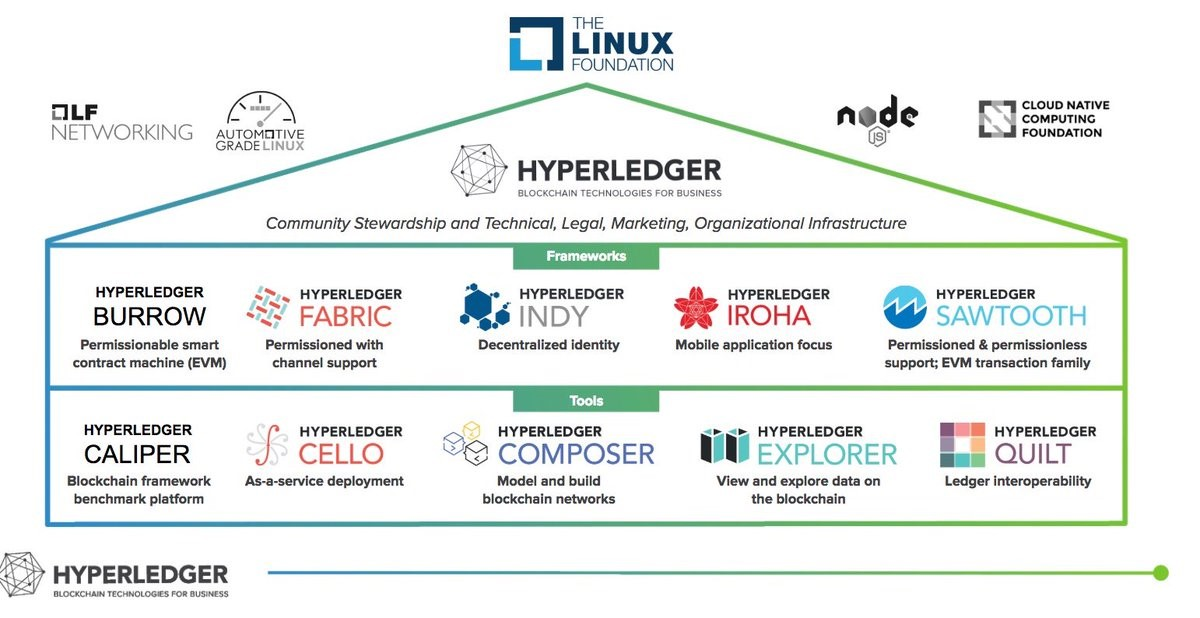
\includegraphics[width=.9\linewidth]{img/hlf_um.jpg}
\caption{Chiến lược Hyperledger Umbrella}
\end{figure}

Nhờ vào thiết kế mô-đun linh hoạt, chính sách quyền hạn cho người tham gia đã giúp Hyperledger Fabric trở thành nền tảng blockchain hoạt động tốt về tốc độ xử lý giao dịch, độ trễ xác nhận giao dịch, cho phép bảo mật và xác minh các giao dịch với hợp đồng thông minh.

\subsection{Những cải tiến của Hyperledger Fabric trong phiên bản 2.x}


Những điểm mới trong phiên bản Hyperledger Fabric 2.x rất thích hợp cho hệ thống mạng blockchain mà đề tài đang hướng đến. Phiên bản mới Fabric 2.x được hỗ trợ dài hạn, điều đó có nghĩa rằng các vấn đề bảo mật, lỗi hệ thống sẽ sớm được công đồng và nhà phát triển cập nhật cho đến khi một phiên bản LTS mới được phát hành.

\begin{figure}[htbp]
\centering
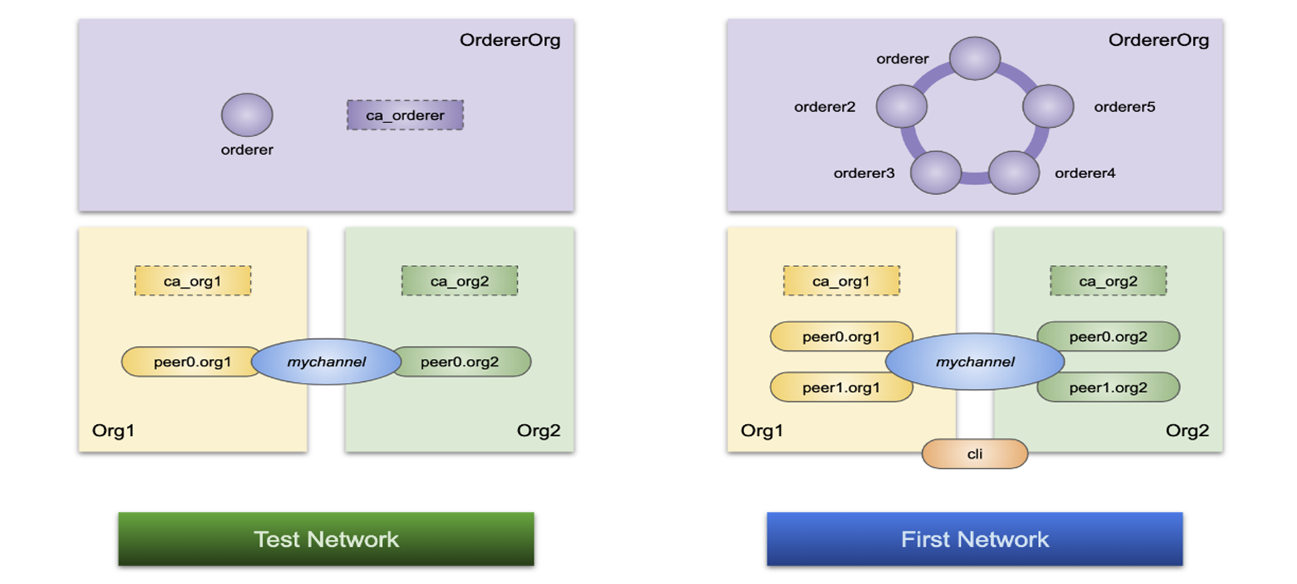
\includegraphics[width=.9\linewidth]{img/hlf_network.png}
\caption{Cấu trúc mạng đề xuất của hai phiên bản 1.4 và 2.x}
\end{figure}

Trong phiên bản Fabric 2.x, các hợp đồng thông minh (chaincode) muốn được cài đặt trên peer và chạy trên channel cần phải thông qua một vòng đời mới. Các tổ chức thuộc kênh (channel) cần thống nhất (đồng ý thõa thuận) các tham số của hợp đồng như chính sách chứng thực hợp đồng trước khi hợp đồng được thực hiện tương tác với sổ cái (ledger).

Việc nâng cấp các hợp đồng thông minh (chaincode) sẽ được gắn với quá trình đồng thuận và chỉ hoàn thành khi đạt được ngưỡng cho phép của các thành viện thuộc kênh. Điều đó có nghĩa tất cả thành viên thuộc kênh luôn giữ đầy đủ các hợp đồng (được cài đặt chaincode) cùng nhau thay vì có thể từ chối như phiên bản 1.4. Việc thay đổi cơ chế nâng cấp giao dịch của phiên bản 2.x mang lại tính an toàn, đồng nhất dữ liệu so với phiên bản trước.

Dữ liệu riêng tư (Data Privacy) cho phép một phần dữ liệu được chia sẽ riêng tư giữa một số thành viên thuộc kênh thay vì tất cả thành viên đều có thể sở hữu. Thay vì tạo thêm một kênh để nhóm các thành viên và mất rất nhiều thời gian để cấu hình (kênh, chính sách, MSP,…) 

Một trong những điểm nổi bật của phiên bản Fabric 2.x là tối ưu hóa hiệu suất hoạt động của mạng Blockchain. Bằng cách thay thế giải thuật Rafka thành giải thuật Raft, thêm một bộ nhớ đệm mới vào các peer để tìm nạp dữ liệu nhanh hơn khi sử dụng CouchDB bên ngoài, xác thực giao dịch song song, xử lý khối bất động bộ, phân trang chaincode,…Điều đó cho phép Hyperledger Fabric 2.x đảm bảo hiệu suất có thể xử lý hàng nghìn giao dịch mỗi giây. 

\subsection{Các thành phần của mạng Hyperledger Fabric}

\textbf{Ledger}: Một quyển sổ cái bao gồm 2 thành phần có liên quan nhau là “blockchain” và “cơ sở dữ liệu trạng thái”. Các giao dịch thay đổi các tài sản(dữ liệu có cấu trúc) của mạng sẽ được “blockchain” ghi nhận theo dạng nhật ký và không thể xóa hay chỉnh sửa. Ngược lại, “cơ sở dữ liệu trạng thái” (LevelDB hoặc CouchDB) lưu trạng thái mới nhất của các tài sản hiện có trong mạng theo cặp giá trị key-value. Ledgers được lưu trên các Peer trong cùng Channel đồng bộ khi có phát sinh giao dịch thông qua cơ chế đồng thuận.

\textbf{Smart contract} (Chaincode): Hợp đồng thông minh – một ứng dụng được viết bằng các ngôn ngữ lập trình như: Javascript, Go, Java dùng để tương tác với mạng, quản lý tài sản. Trong Hyperledger Fabric, các hợp đồng thông minh được gọi là chaincode, được cài đặt trên các Peer.

\textbf{Peer nodes}: Là thành phần cơ bản của mạng, lưu trữ bản sao của Ledgers và thực thi Smart contract. Các peer được quản lý và duy trì bởi các thành viên trong mạng. Peer được chia làm 2 dạng:

\begin{itemize}
\item \textbf{Endorsing peer}: thực thi các giao dịch trong chaincode và đề xuất giao dịch.
\item \textbf{Committing peer}: có thể không cần cài đặt chaincode, lưu trữ sổ cái đầy đủ.
\end{itemize}

\textbf{Ordering Service (Solo, Raft, Kafka)}: Là thành phần chứa thuật toán đồng thuận và đảm nhận nhiệm vụ xác minh, bảo mật, kiểm định chính sách, quản lý cấu hình Channel.

\textbf{Channel}: Kênh là một “mạng con” riêng kết nối giữa hai hoặc nhiều thành viên trong mạng. Cấu hình một kênh gồm các Orgs(tổ chức), Peer, Ledger, Chaincode, Ordering service. Mỗi Peer có thể tham gia nhiều kênh và sẽ được cấp các định danh riêng với từng kênh bởi nhà cung cấp dịch vụ thành viên (MSP).

\textbf{Fabric Certificate Authorities}: Hyperledger Fabric CA là thành phần phát hành chứng chỉ mặc định, cung cấp chứng chỉ dựa trên PKI cho các tổ chức thành viên mạng và người dùng. CA phát hành một chứng chỉ gốc (rootCert) cho mỗi thành viên và một chứng nhận đăng ký (ECert) cho mỗi người dùng được uỷ quyền.

\textbf{Membership Service Provider (MSP)}: Trong cơ sở hạ tầng của mạng  Hyperledger Fabric, MSP là một tập hợp các thư mục được thêm vào cấu hình của mạng Fabric nhằm xác minh một tổ chức. Đây là một tập hơp các thư mục chứa các chứng chỉ số ( cấp từ CA ), giúp mạng Fabric có thể xác thực các thực thể kết nối với mạng thông qua danh tính (Identities) mà không cần khóa bí mật. Ngoài ra, nó còn có vai trò xác định thực đặc quyền truy cập trong phạm vi mạng và kênh của một thành phần nào đó trong mạng.